%\makeatletter
%\def\@makechapterhead#1{%
  %\vspace*{50\p@}%
%  {\parindent \z@ \raggedright \normalfont
%    \interlinepenalty\@M
%    \huge\bfseries  \thechapter.\quad #1\par\nobreak
%    \vskip 20\p@
%  }}
%\makeatother
\chapter{Pair Energy in Isolated Flat Band Limit}\label{App:Pair_Energy}

This appendix presents the expressions derived in \cite{Torma} for the interaction energy shift to a pair of particles in the flat band. By assuming that the flat band is isolated from the other bands by an energy gap $\gg U$, the two-particle eigenstates can justifiably be expanded only in terms of the single-particle flat band Bloch states. As there is no external potential with a different periodicity to the lattice, the total momentum of the particles, $\textbf{q}=\textbf{k}_1+\textbf{k}_2$, is conserved, and is therefore a good quantum number which can be used to label the eigenstates. The energy shifts relative to the flat band, $\Delta E_{\textbf{q}}$, are found to satisfy the eigenvalue equation:
\begin{subequations}\label{Eq:PairEnergy_Eigenvalue}
    \begin{equation}
        \sum_{\textbf{k}'}V_{\textbf{k}\textbf{k}'}(\textbf{q}) A_{\textbf{k}'}=\Delta E_{\textbf{q}}A_{\textbf{k}}
    \end{equation}
    \begin{equation}
        V_{\textbf{k}\textbf{k}'}(\textbf{q})=\frac{U}{N_c}\sum_{\alpha} m_{\textbf{k}',\alpha}^{*} m_{\textbf{q}-\textbf{k}',\alpha}^{*} m_{\textbf{k},\alpha} m_{\textbf{q}-\textbf{k},\alpha}
    \end{equation}
\end{subequations}
with $m_{\textbf{k},\alpha}$ the flat band eigenvector components defined in Eq. \ref{Eq:FBEigenvector} (the label $^{(3)}$ is omitted). Most eigenvalues of $V_{\textbf{k}\textbf{k}'}$ are zero, corresponding to the unperturbed non-overlapping flat band states. $V_{\textbf{k}\textbf{k}'}$ can be approximated by:
\begin{equation}\label{Eq:Approximate_Potential}
    V_{\textbf{k}\textbf{k}'}(\textbf{q})\approx V_{\textbf{k}\textbf{k}'}'(\textbf{q}) = \frac{U}{N_c}\frac{1}{N_{\text{orb}}} (\textbf{m}_{\textbf{k}'}^{*} \cdot \textbf{m}_{\textbf{q}-\textbf{k}'}^{*}) (\textbf{m}_{\textbf{k}} \cdot \textbf{m}_{\textbf{q}-\textbf{k}})
\end{equation}
where $N_{\text{orb}}$ is the number of orbitals in each unit cell ($N_{\text{orb}}=3$ for the kagome lattice). This enables the eigenvalue equation \ref{Eq:PairEnergy_Eigenvalue} to be solved to give:
\begin{equation}\label{Eq:Approximate_Pair_Energy}
    \Delta E_{\textbf{q}}=\frac{U}{N_c}\frac{1}{N_{\text{orb}}}\sum_{\textbf{k}}|\textbf{m}_{\textbf{k}} \cdot \textbf{m}_{\textbf{q}-\textbf{k}}|^2
\end{equation}
Since this expression is the trace of the approximated interaction matrix $V_{\textbf{k}\textbf{k}'}'$, all other eigenvalues of $V_{\textbf{k}\textbf{k}'}'$ are zero.

Fig. \ref{Fig:FB_Analytical_Energy_Shifts} below compares (i) the numerically obtained eigenvalues of the full Hamiltonian (as in Fig. \ref{Fig:Energy_Shifts}), (ii) the numerically obtained eigenvalues of $V_{\textbf{k}\textbf{k}'}$, and (iii) the energies calculated using Eq. \ref{Eq:Approximate_Pair_Energy}, for a 10$\times$10 unit cell system and $U/J=0.1$. Since the isolated flat band condition is not satisfied for the kagome lattice, there is some admixture of dispersive states in the exact case (i); however, the resultant errors in the case (ii) values are minor. Case (iii) involves the additional approximation of $V_{\textbf{k}\textbf{k}'}$ by $V_{\textbf{k}\textbf{k}'}'$, and only gives a single energy value for each $q$; despite this, these values agree extremely closely with the largest eigenvalues of $V_{\textbf{k}\textbf{k}'}$.

\vspace{1cm}

\begin{figure}[ht]
    \centering
    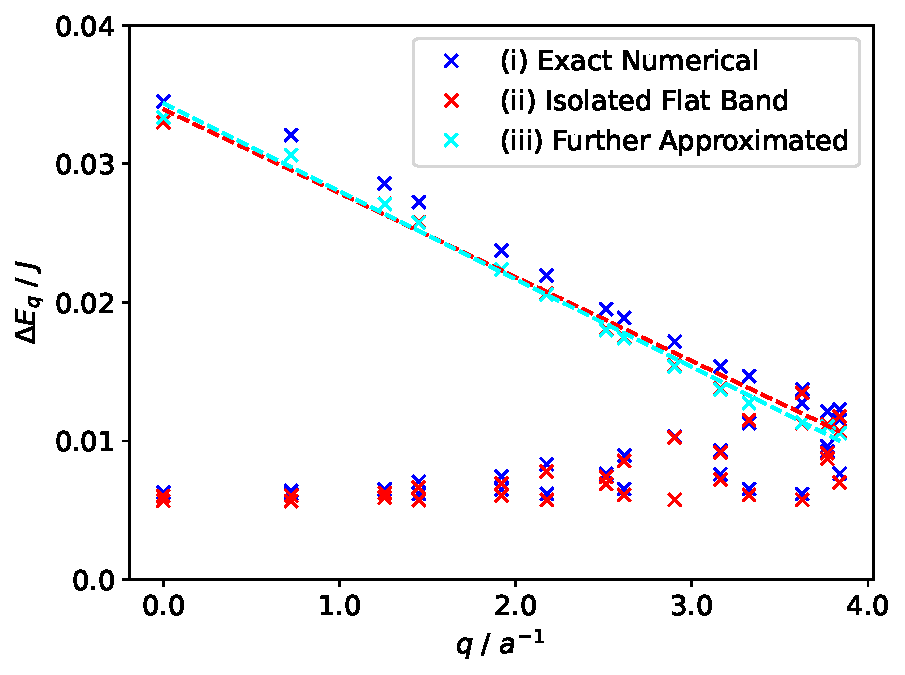
\includegraphics[width=10cm]{Figures/FB_Analytical_Energy_Shifts}
    \caption{Energy shifts of bound particle pairs relative to the flat band energy level, for $U/J=0.1$ in a 10$\times$10 unit cell system, plotted against magnitude of total momentum $q$. Numerical eigenvalues from diagonalizing the full Hamiltonian are shown in dark blue; eigenvalues of the interaction matrices $V_{\textbf{k}\textbf{k}'}(\textbf{q})$ (Eq. \ref{Eq:PairEnergy_Eigenvalue}) in red; energies calculated from Eq. \ref{Eq:Approximate_Pair_Energy} in light blue. Note that these light blue points are almost coincident with the highest of the red points at each $q$. Linear fits to the highest energy values at each $q$ are shown dashed in the respective colours of the datasets.}
    \label{Fig:FB_Analytical_Energy_Shifts}
\end{figure}

For both case (ii) and (iii), the highest-energy eigenvalues have approximately the same gradient as the exact spectrum, and therefore can be used to accurately estimate the group velocity. Linear fits to the data were performed to obtain the respective group velocities, (ii) $v_g=(6.1\pm 0.2)\times 10^{-3}\:a/t_0$ and (iii) $v_g=(6.4\pm 0.1)\times 10^{-3}\:a/t_0$. These closely match the values obtained previously in Section \ref{Sec:HexagonQuantitative}: $v_g=(6.3 \pm 0.2)\times 10^{-3}\: a/t_0$ from the exact eigenspectrum, and $v_g=(6.33 \pm 0.05)\times 10^{-3} \: a/t_0$ from the simulation. In fact, the value from the case (iii) turns out to be more accurate despite the additional approximations involved.

In practice, the expressions throughout this appendix are of limited use for performing dynamical simulations, as in this project. As Appendix \ref{App:Timing} will describe, calculating observables from the state $|\Psi\rangle$, not the time-evolution to find $|\Psi(t)\rangle$, is frequently the computationally limiting step of the simulations. Hence, these approximate expressions may enable faster calculation of the energies and time-evolution, but do not significantly improve the computational capabilities. Instead, they are useful for evaluating quantities which depend only on the eigenspectrum. These include the group velocity, as illustrated above, and the effective mass of the bound particle pairs, as is done in \cite{Torma}.